\section{Experiments}

\subsection{Experimental Setup}

\begin{table*}[t]
  \centering
  \begin{minipage}[b]{0.67\textwidth}
    \vspace{0pt}
    \centering
    \scriptsize
    \renewcommand{\arraystretch}{1.08}
    \setlength{\tabcolsep}{2.4pt}
    \resizebox{\linewidth}{!}{%
    \begin{tabular}{l|cccccccccc|c}
      \hline
      \multicolumn{1}{c|}{\textbf{Model}} & \textbf{OP} & \textbf{CR} & \textbf{CS} & \textbf{ATP} & \textbf{EU} & \textbf{TR} & \textbf{PR} & \textbf{SU} & \textbf{ACP} & \textbf{CT} & \textbf{Avg.} \\
      \hline
      \rowcolor{softred}
      \multicolumn{12}{c}{\textbf{Proprietary models}} \\
      \hline
      GPT-4o & 77.1 & 80.5 & 83.9 & 76.5 & 70.2 & 83.8 & 66.7 & 62.2 & 69.1 & 49.2 & 73.3 \\
      Gemini-1.5-Pro & 79.0 & 80.5 & 83.5 & 79.7 & 80.0 & 84.7 & 77.8 & 64.2 & 72.0 & 48.7 & 75.7 \\
      \hline
      \rowcolor{softorange}
      \multicolumn{12}{c}{\textbf{Open-source offline models}} \\
      \hline
      LLaVA-OV-7B & 80.4 & 74.2 & 76.0 & 80.7 & 72.7 & 71.7 & 67.6 & 65.5 & 65.7 & 45.1 & 71.1 \\
      Qwen2.5-VL-7B & 77.9 & 76.6 & 78.6 & 80.9 & 76.7 & 77.0 & 80.6 & 65.5 & 65.7 & 52.9 & 73.3 \\
      Qwen3-VL-8B & 80.1 & 76.6 & 81.1 & 81.1 & 77.0 & 73.2 & 80.6 & 63.4 & 68.8 & 57.0 & 74.1 \\
      MiniCPM-o-4.5-9B & 80.9 & \textbf{88.3} & 82.0 & 85.0 & 78.9 & 85.4 & 78.7 & 67.1 & 75.6 & \textbf{56.0} & 78.2 \\
      \hline
      \rowcolor{softgreen}
      \multicolumn{12}{c}{\textbf{Open-source streaming models}} \\
      \hline
      Flash-VStream-7B & 25.9 & 43.6 & 24.9 & 23.9 & 27.3 & 13.1 & 18.5 & 25.2 & 23.9 & 48.7 & 23.2 \\
      VideoLLM-online-8B & 39.1 & 40.1 & 34.5 & 31.1 & 46.0 & 32.4 & 31.5 & 34.2 & 42.5 & 27.9 & 36.0 \\
      Dispider-7B & 74.9 & 75.5 & 74.1 & 73.1 & 74.4 & 59.9 & 76.1 & 62.9 & 62.2 & 45.8 & 67.6 \\
      ViSpeak-7B & 79.8 & 71.1 & 81.4 & 78.8 & 74.5 & 70.1 & 63.9 & 64.2 & 71.4 & 28.0 & 70.4 \\
      TimeChat-Online-7B & 80.2 & 82.0 & 79.5 & 83.3 & 76.1 & 78.5 & 78.7 & 64.6 & 69.6 & 58.0 & 75.4 \\
      StreamBridge-7B & 84.7 & 82.7 & 88.9 & 89.8 & 77.4 & 85.4 & \textbf{84.3} & 69.9 & 71.7 & 35.8 & 77.0 \\
      StreamForest-7B & 83.1 & 82.8 & 82.7 & 84.3 & 77.5 & 78.2 & 76.9 & 69.1 & 75.6 & 54.4 & 77.3 \\
      \rowcolor{softblue}
      WTI-8B (Ours) & \textbf{88.1} & 79.7 & \textbf{92.7} & \textbf{90.1} & \textbf{79.2} & \textbf{92.5} & 82.4 & \textbf{80.9} & \textbf{83.2} & 40.4 & \textbf{83.3} \\
      \hline
    \end{tabular}}
    \captionof{table}{StreamingBench real-time visual understanding results.}
    \label{tab:streamingbench_main}
  \end{minipage}
  \hfill
  \begin{minipage}[b]{0.30\textwidth}
    \vspace{0pt}
    \centering
    \scriptsize
    \renewcommand{\arraystretch}{1.08}
    \setlength{\tabcolsep}{2.2pt}
    \resizebox{\linewidth}{!}{%
    \begin{tabular}{@{}l|cccc@{}}
      \hline
      \multicolumn{1}{c|}{\multirow{2}{*}{\textbf{Model}}} & \multirow{2}{*}{\textbf{MLVU}} & \multicolumn{2}{c}{\textbf{V-MME}} & \multirow{2}{*}{\textbf{LVB}} \\
      \cline{3-4}
      & & \textbf{All} & \textbf{Long} & \\
      \hline
      \rowcolor{softorange}
      \multicolumn{5}{c}{\textbf{Offline models}} \\
      \hline
      LongVA-7B & 56.3 & 52.6 & 47.6 & 56.3 \\
      LLaVA-OV-7B & 64.7 & 58.2 & -- & -- \\
      LongVU-7B & 65.4 & 60.6 & -- & -- \\
      Qwen3-VL-8B & 66.7 & 63.5 & 56.3 & 60.7 \\
      \hline
      \rowcolor{softgreen}
      \multicolumn{5}{c}{\textbf{Streaming models}} \\
      \hline
      Dispider-7B & 61.7 & 57.2 & -- & -- \\
      Flash-VStream-7B & 66.3 & 61.2 & -- & -- \\
      StreamForest-7B & \textbf{70.0} & 61.4 & -- & -- \\
      TimeChat-Online-7B & 65.4 & 62.5 & 48.4 & 55.4 \\
      StreamBridge-7B & 69.6 & 64.4 & -- & -- \\
      \rowcolor{softblue}
      WTI-8B (Ours) & 69.9 & \textbf{66.9} & \textbf{58.2} & \textbf{62.9} \\
      \hline
    \end{tabular}}
    \captionof{table}{Offline long-video benchmark results.}
    \label{tab:offline_main}
  \end{minipage}
\end{table*}


\noindent \textbf{Implementation Details.}
WTI is initialized from Qwen3-VL-8B-Instruct~\citep{qwen3vl2025}.
Masked SFT trains on chunk-level trajectories with the vision encoder frozen and updates the language model and multimodal projector at a learning rate of $1\times10^{-5}$.
Stream-GDPO starts from the SFT checkpoint and uses veRL~\citep{sheng2024hybridflow} for one epoch on 8 H20 GPUs, with prompt batch size 64, 4 rollouts per prompt, actor learning rate $1\times10^{-5}$, asymmetric clipping with $\epsilon_{\mathrm{low}}=0.2$ and $\epsilon_{\mathrm{high}}=0.28$, and action-branch loss weight 0.15.
Videos are streamed as 1-second chunks at 2 FPS, and compact-and-reprefill is triggered at the active-context boundary during inference.

\noindent \textbf{Benchmarks.}
We evaluate streaming understanding on StreamingBench and OVO-Bench, reporting the real-time visual understanding split for StreamingBench and Real-Time, Backward, Forward, and weighted overall accuracy for OVO-Bench~\citep{streamingbench2024,ovobench2025}.
We further evaluate Video-MME~\citep{videomme2025}, MLVU~\citep{mlvu2024}, and LongVideoBench~\citep{longvideobench2024} with their official aggregate metrics to test general long-video ability beyond streaming benchmarks.

\noindent \textbf{Baselines.}
We compare with proprietary models, offline/static Video-LLMs, and online or streaming Video-LLMs.
The baselines include GPT-4o and Gemini-1.5-Pro~\citep{openai_gpt4o2024,gemini15_2024}; LongVA, LongVU, LLaVA-series models, Qwen2.5-VL, Qwen3-VL, and MiniCPM-o~\citep{longva2024,longvu2025,llavaonevision2024,llavavideo2024,llavanextvideo2024,qwen25vl2025,qwen3vl2025,minicpmo45_2026}; and VideoLLM-Online, Dispider, ViSpeak, TimeChat-Online, Flash-VStream, StreamBridge, StreamForest, and Streamo~\citep{videollm_online2024,dispider2025,vispeak2025,timechat2024,flashvstream2025,streambridge2025,streamforest2025,streamo2026}.
All online evaluations are causal, and offline/static baselines are restricted to the observed prefix in online benchmarks following the benchmark protocol.

\subsection{Main Results}

We first evaluate whether WTI supports the streaming regimes introduced in Section~\ref{sec:data}: Real-Time and Backward Tracing questions, together with future-dependent Proactive questions that correspond to the Forward category in OVO-Bench.
On OVO-Bench, WTI achieves 73.6\% overall accuracy, outperforming StreamBridge-7B (62.6\%) and ViSpeak-7B (61.1\%), with 76.9\% on Real-Time, 73.4\% on Backward, and 70.0\% on Forward.
This pattern is consistent with WTI's online design: time-indexed memory and recall support Backward reasoning over previously observed chunks, while active-window perception and multi-turn textual state preserve Real-Time and Forward answering.
The best OVO overall score among open-source streaming baselines suggests that history-aware recall improves long-context streaming reasoning without weakening current-prefix perception.

StreamingBench further supports this result at a finer RTVU granularity.
WTI reaches 83.3\% average accuracy, compared with 77.3\% for StreamForest-7B and 77.0\% for StreamBridge-7B.
WTI leads on OP, CS, ATP, EU, TR, SU, and ACP, suggesting strong active-window perception and temporal state tracking; CT remains the main weak category, indicating that fine-grained temporal aggregation is still challenging under a bounded streaming state.
On offline long-video benchmarks, WTI obtains 66.9\% on Video-MME, 58.2\% on Video-MME Long, and 62.9\% on LongVideoBench, while matching StreamForest-7B on MLVU with 69.9\% vs. 70.0\%.
Overall, WTI improves history-dependent reasoning through compact memory and recall while preserving current-prefix, Forward, and offline long-video performance.

\begin{figure*}[t]
  \centering
  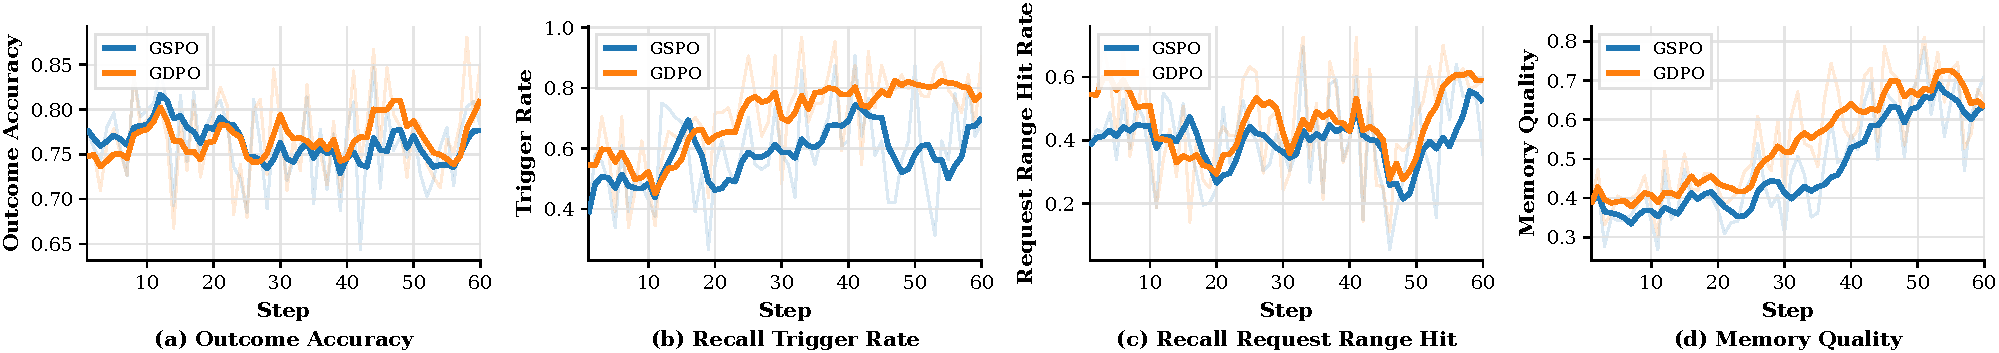
\includegraphics[width=0.98\textwidth]{figures/ablation/gspo_gdpo_step_comparison.pdf}
  \caption{Training-time GSPO/GDPO diagnostics. Panels report outcome accuracy, BT recall trigger rate, post-recall outcome accuracy, and memory quality; faint and bold curves show raw and rolling values.}
  \label{fig:gspo_gdpo_step_comparison}
  \vspace{0.2em}
  \makebox[\textwidth][c]{%
  \begin{minipage}[t]{\dimexpr(\textwidth-\columnsep)/2\relax}
    \vspace{0pt}
    \centering
    \scriptsize
    \renewcommand{\arraystretch}{1.12}
    \setlength{\tabcolsep}{2.0pt}
    \makebox[\linewidth][c]{\resizebox{0.98\linewidth}{!}{%
    \begin{tabular}{@{}l|cccccccc@{}}
      \hline
      \multirow{2}{*}{\textbf{Config}} & \multirow{2}{*}{\textbf{Streaming}} & \multicolumn{4}{c}{\textbf{OVO-Bench}} & \multicolumn{3}{c}{\textbf{Long-video}} \\
      \cline{3-6}\cline{7-9}
      & & \textbf{RT} & \textbf{BT} & \textbf{FT} & \textbf{Avg.} & \textbf{V-MME} & \textbf{MLVU} & \textbf{LVB} \\
      \hline
      Base model & 74.1 & 64.8 & 54.4 & 63.5 & 61.4 & 63.5 & 66.7 & 60.7 \\
      + SFT & 75.3 & 74.2 & 60.3 & 60.9 & 65.7 & 64.7 & 67.6 & 59.8 \\
      + GSPO & 80.0 & 76.2 & 65.3 & 60.7 & 67.8 & 65.6 & 68.7 & 61.7 \\
      \rowcolor{softblue}
      + GDPO & \textbf{83.3} & \textbf{76.9} & \textbf{73.4} & \textbf{70.0} & \textbf{73.6} & \textbf{66.9} & \textbf{69.9} & \textbf{62.9} \\
      \hline
    \end{tabular}}}
    \captionof{table}{Training objective ablation.}
    \label{tab:training_objective_ablation}
  \end{minipage}%
  \hspace{\columnsep}%
  \begin{minipage}[t]{\dimexpr(\textwidth-\columnsep)/2\relax}
    \vspace{0pt}
    \centering
    \scriptsize
    \renewcommand{\arraystretch}{1.12}
    \setlength{\tabcolsep}{2.0pt}
    \makebox[\linewidth][c]{%
    \begin{tabular}{@{}lcccc@{}}
      \hline
      \textbf{Variant} & \textbf{OVO-BT} & \textbf{V-MME} & \textbf{MLVU} & \textbf{LVB} \\
      \hline
      \rowcolor{softblue}
      Full & 73.4 & 66.9 & 69.9 & 62.9 \\
      w/o memory & 62.8 & 63.5 & 44.7 & 61.6 \\
      w/o recall & 55.5 & 48.3 & 54.2 & 57.9 \\
      memory only & 48.2 & 47.7 & 46.5 & 57.1 \\
      \hline
    \end{tabular}}
    \captionof{table}{Component ablation summary.}
    \label{tab:component_ablation_summary}
  \end{minipage}%
  }
\end{figure*}

\subsection{Ablations}

Table~\ref{tab:training_objective_ablation} separates protocol initialization from trajectory-level policy optimization.
Masked SFT raises StreamingBench from 74.1\% to 75.3\% and OVO-RT from 64.8\% to 74.2\%, showing that the model learns the basic action format and recent-prefix perception.
However, OVO-BT improves more modestly to 60.3\%, and OVO-FT reaches 60.9\%, below the base model's 63.5\%.
This indicates that imitation alone improves recent-prefix perception but does not sufficiently optimize recall timing, compact-memory quality, or exact delayed answering for future-dependent queries.

Figure~\ref{fig:gspo_gdpo_step_comparison} explains why Stream-GDPO improves this behavior over GSPO~\citep{zheng2025gspo}.
Although raw curves are noisy, GDPO maintains stronger BT recall triggering, higher post-recall outcome accuracy, and better memory quality.
Higher memory quality suggests less information loss during compression, while stronger post-recall outcomes indicate that retrieved evidence is more often converted into correct answers.
Accordingly, GDPO raises OVO-BT from 65.3\% to 73.4\% and OVO-FT from 60.7\% to 70.0\% over GSPO, lifting the overall score to 73.6\%.

Table~\ref{tab:component_ablation_summary} shows that compact memory and recall are complementary rather than interchangeable.
Removing memory lowers OVO-BT from 73.4\% to 62.8\%, while removing recall lowers it to 55.5\%; the memory-only variant reaches only 48.2\%.
Thus, memory lines are useful as compact indices, but the model still needs recall to reopen visual evidence for fine-grained historical questions.
The offline ablations follow the same pattern, with w/o recall reducing Video-MME from 66.9\% to 48.3\% and w/o memory reducing MLVU from 69.9\% to 44.7\%.
Together, the ablations show that WTI works because SFT builds the protocol, GDPO trains the online policy, memory preserves bounded history, and recall restores precise evidence when needed.

\FloatBarrier
